\documentclass[notes=show]{beamer}


%%%%%%%%%%%%%%%%%%%%%%%%%%%%%%%%%%%%%%%%%%%%%%%%%%%%%%%%%%%%%%%%%%%%%%%%%%%%%%%%%%%%%%%%%%%%%%%%%%%
%Load additional packages for more flexbility in designing slides
\usepackage{mathptmx}
\usepackage{lmodern}
\usepackage[latin9]{inputenc}
\usepackage{color}
\usepackage{amsmath}
\usepackage{graphicx}
\usepackage{amssymb}
\usepackage{colortbl}
\usepackage{dsfont}
\usepackage{epstopdf}
\usepackage{soul} %%% pt \hl{} (highlight)
\usepackage{bbm}
\usepackage{natbib}
\usepackage{multicol}
\usepackage{eurosym}
\usepackage{booktabs}
\usepackage{array}
\usepackage{color, colortbl}
\usepackage[absolute,overlay]{textpos}
\usepackage{setspace}
\newcommand\FrameText[1]{%
	\begin{textblock*}{\paperwidth}(0pt,\textheight)
		\raggedleft #1\hspace{.5em}
\end{textblock*}}
\usepackage{mathpazo}
\usepackage{hyperref}
\usepackage{multimedia}
\usepackage{datetime}
\usepackage{wrapfig}
\usepackage{comment}

%%%%%%%%%%%%%%%%%%%%%%%%%%%%%%%%%%%%%%%%%%%%%%%%%%%%%%%%%%%%%%%%%%%%%%%%%%%%%%%%%%%%%%%%%%%%%%%%%%%



%%%%%%%%%%%%%%%%%%%%%%%%%%%%%%%%%%%%%%%%%%%%%%%%%%%%%%%%%%%%%%%%%%%%%%%%%%%%%%%%%%%%%%%%%%%%%%%%%%%
\definecolor{light-gray}{gray}{0.75}
\definecolor{lgray}{gray}{0.5}
\definecolor{Gray}{gray}{0.8}

%MODIFY THE STANDARD SLIDE LAYOUT
\usetheme{Madrid}
\setbeamercovered{invisible}
\setbeamertemplate{navigation symbols}{}
\newcounter{MyCounter}
\setbeamertemplate{section in toc}
{\edef\DefTemp{\noexpand\setcounter{MyCounter}{\inserttocsectionnumber}}
	\DefTemp\Roman{MyCounter}
	\inserttocsection
	\par}
\setbeamertemplate{caption}[numbered]

%MODIFY THE SLIDE FOOTLINE
\setbeamertemplate{footline}
{\hbox{
		\begin{beamercolorbox}[wd=.33333\paperwidth,ht=2.25ex,dp=1ex,center,ignorebg]{author in head/foot}
			\usebeamerfont{author in head/foot}\color{white}\insertshortauthor
		\end{beamercolorbox}
		\begin{beamercolorbox}[wd=.33333\paperwidth,ht=2.25ex,dp=1ex,center,ignorebg]
			{title in head/foot}
			\usebeamerfont{title in head/foot}\color{white}\insertshorttitle
		\end{beamercolorbox}
		\begin{beamercolorbox}[wd=.33333\paperwidth,ht=2.25ex,dp=1ex,right,ignorebg]
			{date in head/foot}
			\usebeamerfont{date in head/foot}\textcolor{white}\insertshortdate\hspace{0.5cm}
			\textcolor{white}{\insertframenumber{} / \inserttotalframenumber} \hspace{0.5cm}
		\end{beamercolorbox}
}}

\makeatletter
\newcommand\makebeamertitle{\frame{\maketitle}}
\AtBeginDocument{
	\let\origtableofcontents=\tableofcontents
	\def\tableofcontents{\@ifnextchar[{\origtableofcontents}{\gobbletableofcontents}}
	\def\gobbletableofcontents#1{\origtableofcontents}
}
\makeatother

\newcommand{\ubcolor}[2]{\color{#1}{\underbrace{\color{black}{#2}}}}
\setbeamercovered{transparent=0}
\setbeamertemplate{items}[square]
\newsavebox{\mybox}
\newcolumntype{G}{@{}>{\begin{lrbox}{\mybox}}l<{\end{lrbox}}@{}} %a column that gobbles its entries
%%%%%%%%%%%%%%%%%%%%%%%%%%%%%%%%%%%%%%%%%%%%%%%%%%%%%%%%%%%%%%%%%%%%%%%%%%%%%%%%%%%%%%%%%%%%%%%%%%%

% Below used to fix issue with notes
\let\orignote\note
\renewcommand{\note}[1]{\orignote{
		\begin{minipage}{\textwidth}
			#1
		\end{minipage}
}}


%\includecomment{undergrad}
\excludecomment{undergrad}
\includecomment{grad}
%\excludecomment{grad}

\begin{document}

\title[Bond Trading]{Bonus Material: Bond Trading}
\begin{undergrad}
\subtitle{FINC 462/662}
\end{undergrad}
\begin{grad}
\subtitle{FINC 462/662}
\end{grad}
\author[M. Fleckenstein]{Matthias Fleckenstein}
\institute[University of Delaware]{University of Delaware, Lerner College of Business and Economics}
\date{Spring 2022}
\maketitle




\setbeamertemplate{footline}
{\hbox{
		\begin{beamercolorbox}[wd=.33333\paperwidth,ht=2.25ex,dp=1ex,center,ignorebg]{author in head/foot}
			\usebeamerfont{author in head/foot}\color{white}\insertshortauthor
		\end{beamercolorbox}
		\begin{beamercolorbox}[wd=.33333\paperwidth,ht=2.25ex,dp=1ex,center,ignorebg]
			{title in head/foot}
			\usebeamerfont{title in head/foot}\color{white}\inserttitle
		\end{beamercolorbox}
		\begin{beamercolorbox}[wd=.33333\paperwidth,ht=2.25ex,dp=1ex,right,ignorebg]
			{date in head/foot}
			\usebeamerfont{date in head/foot}\color{white}\hspace{0.5cm}
			\insertframenumber{} / \inserttotalframenumber \hspace{0.5cm}
		\end{beamercolorbox}
}}

\setcounter{framenumber}{0}


\frame{\frametitle{Introduction}
In this set of slides, we will talk about a few examples:
\begin{itemize}
\item Trading on beliefs
\begin{itemize}
\item Steepener Trade
\item On-the-run/off-the-run
\end{itemize}
\item Hedging liabilities that are sensitive to interest rates
\begin{itemize}
\item Pension fund example
\item Perpetuity
\item Zero initial cash outlay
\end{itemize}
\end{itemize}

}


\section{Trading on Beliefs}

\frame{\frametitle{The Algorithm}
Generally, trading on interest rates requires the following steps:
\begin{enumerate}
\item Identify your views.
\item Calculate measures of interest rate exposure (duration and/or convexity).
\item Determine the correct portfolio to hedge against certain types of interest rate exposures.
\item Verify that you did the trade correctly by doing some scenario analysis.
\end{enumerate}
}


\subsection{Steepener Trade}
\frame{\frametitle{Steepener Trade}
Sometimes our views might be about relative prices -- equivalently, our views may be about relative interest rates.  Let's consider an example.

\begin{itemize}
\item Suppose that the yield on a 2-year bond is 4\% and the yield on a 10-year bond is 6\%.  (both zero coupon bonds; annually compounded yields)
\item Suppose also that we believe that the yield on the 10-year bond will increase \textit{relative} to the yield on the 2-year bond.
\item We are not sure whether the overall level of yields will go up or down.
\end{itemize}
}



\frame{\frametitle{Steepener Trade}
\begin{center}
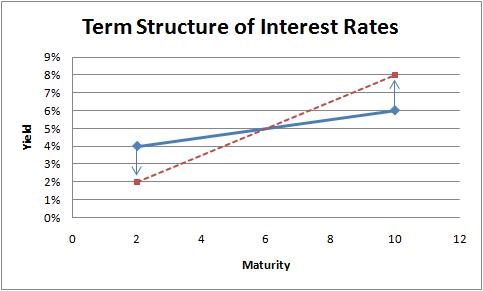
\includegraphics[width=4in]{figures/steepener1.jpg}
\end{center}
}

\note{
\begin{itemize}
\item 10-yr yield $\uparrow \Rightarrow$ Price $\downarrow$
\item 2-yr yield $\downarrow \Rightarrow$ Price $\uparrow$
\item Suggests that we want to long the 2-year and short the 10-yr.
\end{itemize}
}

\begin{undergrad}
\frame{\frametitle{Clicker Question}
What happens to the prices of the 2-year and 10-year bonds if the 2-year yield goes down and the 10-year yield goes up?\\\bigskip
(A) Both prices go up\\\smallskip
(B) Both prices go down\\\smallskip
(C) The 2-year price goes up and the 10-year price goes down\\\smallskip
(D) The 2-year price goes down and the 10-year price goes up\\\smallskip

}

\note{
\begin{itemize}
\item 10-yr yield $\uparrow \Rightarrow$ Price $\downarrow$
\item 2-yr yield $\downarrow \Rightarrow$ Price $\uparrow$
\item Suggests that we want to long the 2-year and short the 10-yr.
\end{itemize}

}
\end{undergrad}

\frame{\frametitle{Steepener Trade}
\begin{center}
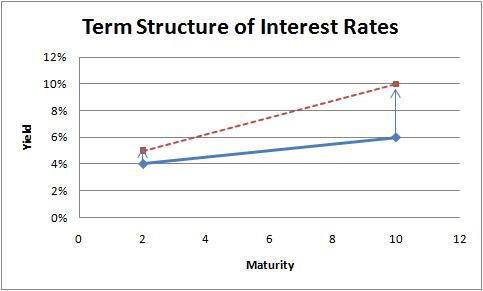
\includegraphics[width=4in]{figures/steepener2.jpg}
\end{center}
}

\note{
\begin{itemize}
\item Both yields go up, but 10yr yield goes up by more.
\item Yield curve is steeper.
\end{itemize}
}

\frame{\frametitle{Steepener Trade}
\begin{center}
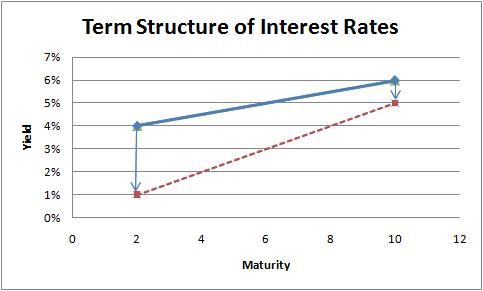
\includegraphics[width=4in]{figures/steepener3.jpg}
\end{center}
}

\note{
\begin{itemize}
\item Both yields go down, but 2yr goes down more.
\item Yield curve is steeper.
\end{itemize}
}

\frame{\frametitle{Steepener Trade}
\begin{center}
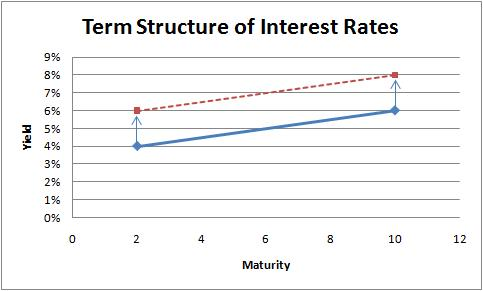
\includegraphics[width=4in]{figures/steepener4.jpg}
\end{center}
}

\note{
\begin{itemize}
\item Move in parallel.
\item Same steepness.
\item Break-even case: To be used to determine the proportion of each bond in the portfolio.
\end{itemize}
}

\frame{\frametitle{Steepener Trade}
\begin{center}
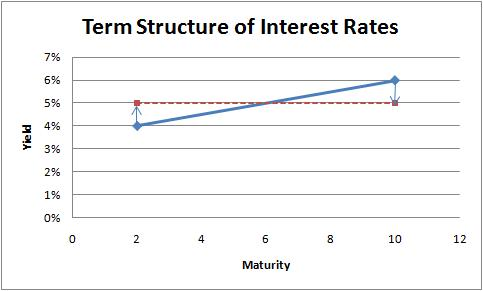
\includegraphics[width=4in]{figures/steepener5.jpg}
\end{center}
}

\note{
\begin{itemize}
\item Flatter
\item Opposite of what we are betting on.  Should expect to lose money.
\end{itemize}
}

\begin{undergrad}
\frame{\frametitle{Steepener Trade}

\begin{itemize}
\item \underline{Step 1}: We think the yield curve will get steeper.  Thus, we want to buy the 2-year bond and short the 10-year bond.

\begin{itemize}
\item But in what proportion? \ We want our exposure to the level of
interest rates to roughly be zero. \ (If the 2-year rate and the 10-year
rate change by the same amount, we want our portfolio value to remain close
to constant.)
\end{itemize}

\item \underline{Step 2}: Some important quantities.
\vspace{1.5in}
\end{itemize}
}

\note{
\begin{itemize}
\item \$1000 face value of the 10-year bond is worth $\frac{\$1000}{%
(1.06)^{10}}=\$558.39$

\item $MD_{10}=\frac{10}{1.06}=9.434$

\item $MD_{2}=\frac{2}{1.04}=1.923$
\end{itemize}

We could have also used the MD approximation formula to calculate MDs.  For the 10-yr:
\begin{align*}
&B(y + \Delta y) = \frac{1000}{1.061^{10}} = 553.1541\\
&B(y - \Delta y) = \frac{1000}{1.059^{10}} = 563.6901\\
&MD_{10} \approx -\frac{553.1541 - 563.6901}{2\times .001}\times \frac{1}{558.39} = 9.434
\end{align*}
}
\end{undergrad}

\begin{grad}
\frame{\frametitle{Steepener Trade}

\begin{itemize}
\item \underline{Step 1}: We think the yield curve will get steeper.  Thus, we want to buy the 2-year bond and short the 10-year bond.

\begin{itemize}
\item But in what proportion? \ We want our exposure to the level of
interest rates to roughly be zero. \ (If the 2-year rate and the 10-year
rate change by the same amount, we want our portfolio value to remain close
to constant.)
\end{itemize}

\item \underline{Step 2}: Some important quantities.
\begin{itemize}
\item \$1000 face value of the 10-year bond is worth $\frac{\$1000}{%
(1.06)^{10}}=\$558.39$

\item $MD_{10}=\frac{10}{1.06}=9.434$

\item $MD_{2}=\frac{2}{1.04}=1.923$
\end{itemize}
\end{itemize}
}

\note{
We could have also used the MD approximation formula to calculate MDs.  For the 10-yr:
\begin{align*}
&B(y + \Delta y) = \frac{1000}{1.061^{10}} = 553.1541\\
&B(y - \Delta y) = \frac{1000}{1.059^{10}} = 563.6901\\
&MD_{10} \approx -\frac{553.1541 - 563.6901}{2\times .001}\times \frac{1}{558.39} = 9.434
\end{align*}

}
\end{grad}

\begin{undergrad}
\frame{\frametitle{Steepener Trade}
\vspace{-0.5in}

\underline{Step 3}: Let's consider a long position in the 2-year of \$x and a short position in
the 10-year of \$558.39 (\$1000 face value):

\bigskip

\begin{center}
\begin{tabular}{p{1.5in}|p{1.5in}}
Assets &  Liabilities \\ \hline
\$x in 2-year  &  \$558.39 in 10-year\\ 
&\\
&\\
&\\
&\\
\end{tabular}
\end{center}
}

\note{
\begin{center}
\begin{tabular}{p{1.5in}|p{1.5in}}
Assets &  Liabilities \\ \hline
\$x in 2-year  &  \$558.39 in 10-year\\ 
$MD_{2}=1.923$ & $MD_{10}=9.434$\\
If yield changes by $\Delta y$:  & If yield changes by $\Delta y$: \\ 
$\frac{\Delta B}{B}\approx -1.923\Delta y $ & $\frac{\Delta B}{B}\approx -9.434\Delta y$\\
x(-1.923) & (558.39)(-9.434)\\
\end{tabular}
\end{center}

\bigskip

Thus, x = \$2739.295 or \$2962.82 in face value of the 2-year bond.

\begin{align*}
2739.295 = \frac{\text{Face value}}{1.04^2}
\end{align*}
}
\end{undergrad}

\begin{grad}
\frame{\frametitle{Steepener Trade}
\vspace{-0.5in}

\underline{Step 3}: Let's consider a long position in the 2-year of \$x and a short position in
the 10-year of \$558.39 (\$1000 face value):

\bigskip

\begin{center}
\begin{tabular}{p{1.5in}|p{1.5in}}
Assets &  Liabilities \\ \hline
\$x in 2-year  &  \$558.39 in 10-year\\ 
$MD_{2}=1.923$ & $MD_{10}=9.434$\\
If yield changes by $\Delta y$:  & If yield changes by $\Delta y$: \\ 
$\frac{\Delta B}{B}\approx -1.923\Delta y $ & $\frac{\Delta B}{B}\approx -9.434\Delta y$\\
x(-1.923) & (558.39)(-9.434)\\
\end{tabular}
\end{center}

\bigskip

Thus, x = \$2739.295 or \$2962.82 in face value of the 2-year bond.
}

\note{
\begin{align*}
2739.295 = \frac{\text{Face value}}{1.04^2}
\end{align*}

}
\end{grad}
\frame{\frametitle{Steepener Trade}
\underline{Step 4}:

\begin{itemize}
\item Overall position value is: \$2180.90

\item Let's see how well we have done in hedging level changes:

\begin{itemize}
\item If $y_{2}\rightarrow 6\%$ and $y_{10}\rightarrow 8\%$ (both yields
increase by 2\%), then the portfolio is worth \$2173.71.

\item If $y_{2}\rightarrow 2\%$ and $y_{10}\rightarrow 4\%$ (both yields
decrease by 2\%), then the portfolio is worth \$2172.21.
\end{itemize}

\item What if the yield curve steepens?

\begin{itemize}
\item If $y_{2}\rightarrow 4\%$ and $y_{10}\rightarrow 8\%$, then the
portfolio is worth \$2276.10.
\end{itemize}
\end{itemize}
}

\note{
\begin{itemize}
\item Overall value = 2739.29 - 558.39 = 2180.90
\item If $y_{2}\rightarrow 6\%$ and $y_{10}\rightarrow 8\%$
\begin{align*}
\frac{2962.82}{1.06^2} - \frac{1000}{1.08^{10}} = 2173.71
\end{align*}
\item If $y_{2}\rightarrow 2\%$ and $y_{10}\rightarrow 4\%$
\begin{align*}
\frac{2962.82}{1.02^2} - \frac{1000}{1.04^{10}} = 2172.21
\end{align*}
\item If $y_{2}\rightarrow 4\%$ and $y_{10}\rightarrow 8\%$
\begin{align*}
\frac{2962.82}{1.04^2} - \frac{1000}{1.08^{10}} = 2276.10
\end{align*}
Gain $\approx$ \$95
\end{itemize}
}

\frame{\frametitle{Steepener Trade Discussed}

\begin{itemize}
\item We can use modified durations to make our portfolio (close to)
insensitive to level changes.

\item This allows us to bet on relative yields.

\item In many ways, this is like a long-short equity strategy.
\end{itemize}
}

\note{
\begin{itemize}
\item Buy what we think is (relatively) too cheap.
\item Short what we think is (relatively) too expensive.
\item Buy in the right proportion to be ``market-neutral."
\end{itemize}
}

\subsection{Fixed Income Arbitrage}
\frame{\frametitle{Fixed Income Arbitrage}

\begin{itemize}
\item One very popular trade is based on on-the-run versus off-the-run US\
Treasury bonds.

\item On-the-run Treasuries are the most recently issued US\ Treasuries.

\item Off-the-run Treasuries are all of the other Treasuries and tend to
have low prices (high yields) relative to on-the-run Treasuries.

\item Buy off-the-run Treasuries and short on-the-run Treasuries.
\end{itemize}

Caution: This trade is not an arbitrage in an academic (free money) sense.
}

\note{

}

\frame{\frametitle{Fixed Income Arbitrage Example}
\begin{center}
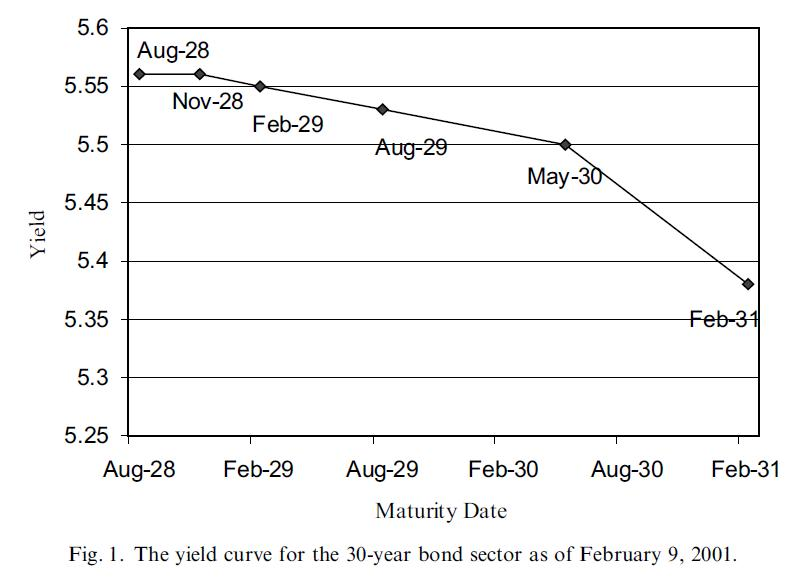
\includegraphics[width=3.5in]{figures/on_the_run.jpg}\\
{\footnotesize Note the difference in yields between the May-30 (29.25yr) and Feb-31 (30yr) bonds.\\
Source: Krishnamurthy (2001)}
\end{center}
}

\note{
\begin{itemize}
\item The idea is that these long maturity bonds are not very different from each other, so their yields should not be very different.
\begin{itemize}
\item Notice the 13 bps gap between May-30 and Feb-31.
\item It just visually looks different.
\end{itemize}
\item We might expect that the yield at the very right will go up a little.
\item Undergrad: Clicker Q on next slide.
\end{itemize}
}

\begin{undergrad}
\frame{\frametitle{Fixed Income Arbitrage Example}
\begin{center}
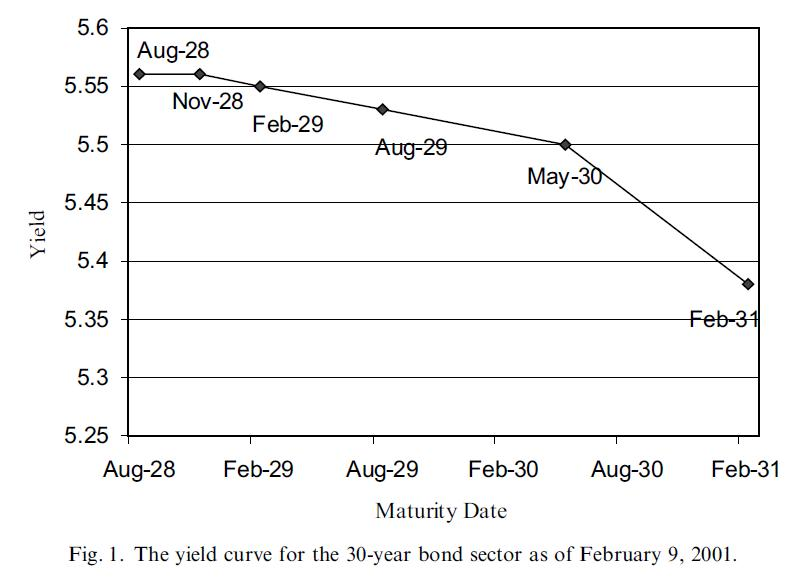
\includegraphics[width=2.5in]{figures/on_the_run.jpg}\\
\vspace{-0.1in}
{\tiny Source: Krishnamurthy (2001)}
\end{center}

{\footnotesize
\underline{Clicker Question}:\\
What is the correct long-short portfolio?\\
(A) Buy the Feb-31 bond and short the May-30 bond\\
(B) Short the Feb-31 bond and buy the May-30 bond\\
(C) Buy both the Feb-31 and May-30 bonds\\
(D) Short both the Feb-31 and May-30 bonds

}
}

\note{

}
\end{undergrad}

\frame{\frametitle{LTCM}
``One of the fund's main strategies was to exploit tiny differences between the price of a newly issued (``on the run") 30-year American Treasury bond, and a similar one issued previously (``off the run").  There is little economic reason for these bonds to have different yields.  Yet off-the-run Treasuries often trade slightly cheaper than on-the-run ones.  LTCM bet that their yields would converge by buying off-the-run Treasuries and selling their on-the-run counterparts short."

\bigskip

- \textit{Economist}, October 17, 1998
}

\note{

}

\begin{undergrad}
\frame{\frametitle{The Trade}
For simplicity, let us assume that the two bonds are both zero-coupon.
\begin{center}
\begin{tabular}{p{1.5in}|p{1.5in}}
Long (Assets) & Short (Liabilities) \\ \hline
\\
\\
\\
\\
\end{tabular}
\end{center}

\vspace{2in}
}

\note{
\begin{center}
\begin{tabular}{l|l}
Long (off-the-run) & Short (on-the-run)\\ \hline
\$x of 29.25yr bond & \$1000 of 30yr bond \\
$MD = \frac{29.25}{1.055} = 27.7251$ & $MD = \frac{30}{1.0538}=28.4684$ \\
$\frac{\Delta B}{B} \approx -27.7251 \Delta y$ & $\frac{\Delta B}{B} \approx -28.4684 \Delta y$\\
\multicolumn{2}{c}{-27.7251x=-28.4684(1000)}
\end{tabular}

\bigskip

x = 1026.81
\end{center}

\underline{Face values}:\\
Off-the-run: $1026.81(1.055)^{29.25} = 4916.14$\\
On-the-run: $1000(1.0538)^{30} = 4816.66$

\bigskip

\underline{Portfolio value}:
1026.81 - 1000 = 26.81

\begin{itemize}
\item The bonds are not actually zero coupon in reality.
\item Remember: On-the-run bond is the expensive one.
\end{itemize}
}
\end{undergrad}

\begin{grad}
\frame{\frametitle{The Trade}
\begin{center}
\begin{tabular}{l|l}
Long (off-the-run) & Short (on-the-run)\\ \hline
\$x of 29.25yr bond & \$1000 of 30yr bond \\
$MD = \frac{29.25}{1.055} = 27.7251$ & $MD = \frac{30}{1.0538}=28.4684$ \\
$\frac{\Delta B}{B} \approx -27.7251 \Delta y$ & $\frac{\Delta B}{B} \approx -28.4684 \Delta y$\\
\multicolumn{2}{c}{-27.7251x=-28.4684(1000)}
\end{tabular}

\bigskip

x = 1026.81
\end{center}

\underline{Face values}:\\
Off-the-run: $1026.81(1.055)^{29.25} = 4916.14$\\
On-the-run: $1000(1.0538)^{30} = 4816.66$

\bigskip

\underline{Portfolio value}:
1026.81 - 1000 = 26.81
}

\note{
\begin{itemize}
\item The bonds are not actually zero coupon in reality.
\item Remember: On-the-run bond is the expensive one.
\end{itemize}
}
\end{grad}

\begin{undergrad}
\frame{\frametitle{Balance Sheet}
\begin{center}
\begin{tabular}{p{1.5in}|p{1.5in}}
Long (Assets) & Short (Liabilities) \\ \hline
\\
\\
\\
\\
\end{tabular}
\end{center}

\vspace{2in}

}

\note{
\begin{center}
\begin{tabular}{l|l}
Long (Assets) & Short (Liabilities) \\ \hline
Off-the-run (29.25yr) bond & On-the-run (30yr) bond\\
\$4916.14 in face value & \$4816.66 in face value\\
\$1026.81 in market value & \$1000 in market value
\end{tabular}
\end{center}

\vspace{2in}

}
\end{undergrad}

\begin{grad}
\frame{\frametitle{Balance Sheet}
\begin{center}
\begin{tabular}{l|l}
Long (Assets) & Short (Liabilities) \\ \hline
Off-the-run (29.25yr) bond & On-the-run (30yr) bond\\
\$4916.14 in face value & \$4816.66 in face value\\
\$1026.81 in market value & \$1000 in market value
\end{tabular}
\end{center}

}

\note{

}
\end{grad}

\frame{\frametitle{Waiting for prices to converge}
Suppose that we wait nine months and the yield of the on-the-run bond goes up to 5.47\% while the yield of the off-the-run bond stays at 5.5\%.

\bigskip

New portfolio value:\\
$\frac{4916.14}{1.055^{28.5}} - \frac{4816.66}{1.0547^{29.25}} = 54.45$

}

\note{
\begin{itemize}
\item Nine months = 0.75 years
\item 5.47\% makes the yield curve linear.
\end{itemize}
}

\section{Hedging}
\subsection{Pension Fund Example}
\frame{\frametitle{Hedging Interest Rate Risk}
\begin{itemize}
\item Suppose that you are managing a pension fund.
\item You have a liability of \$100mm per year for the next 100 years.
\item How do you create a portfolio of Treasury bonds to hedge your exposure to interest rate risk?
\end{itemize}

The US Government does not sell bonds with 100 year maturities, so we cannot just buy bonds with cash flows to match the liability.

}

\note{
\begin{itemize}
\item Disney did issue a 100-yr bond known widely as the ``Sleeping Beauty Bond."
\end{itemize}
}

\begin{undergrad}
\frame{\frametitle{Managing a Pension Fund}
Let's first value the pension liability.  It's an annuity.  Let's assume that the discount rate is 5\% regardless of maturity (term structure is flat).

\vspace{1.75in}

Let's also suppose that the pension fund currently has \hspace{0.75in} in cash.  That is, the pension fund is neither under- nor overfunded.
}

\note{
\begin{align*}
\text{Value of Liability} &= 100\times \frac{1}{0.05}\left[1 - \frac{1}{1.05^{100}}\right]\\
&= 1984.79102
\end{align*}

\begin{itemize}
\item In reality, it's difficult to determine a default-free yield for $T>30$.
\begin{itemize}
\item Most models suggest that yields are mean-reverting, so we might just take a long-run average.
\item Vasicek: $dr_t = \kappa (\theta - r_t) dt + \sigma_r dZ_t$
\end{itemize}
\item Underfunding has been a major issue for a lot of state pension plans.
\end{itemize}
}
\end{undergrad}

\begin{grad}
\frame{\frametitle{Managing a Pension Fund}
Let's first value the pension liability.  It's an annuity.  Let's assume that the discount rate is 5\% regardless of maturity (term structure is flat).

\begin{align*}
\text{Value of Liability} &= 100\times \frac{1}{0.05}\left[1 - \frac{1}{1.05^{100}}\right]\\
&= 1984.79102
\end{align*}

Let's also suppose that the pension fund currently has 1984.79102 in cash.  That is, the pension fund is neither under- nor overfunded.
}

\note{
\begin{itemize}
\item In reality, it's difficult to determine a default-free yield for $T>30$.
\begin{itemize}
\item Most models suggest that yields are mean-reverting, so we might just take a long-run average.
\item Vasicek: $dr_t = \kappa (\theta - r_t) dt + \sigma_r dZ_t$
\end{itemize}
\item Underfunding has been a major issue for a lot of state pension plans.
\end{itemize}
}
\end{grad}

\begin{undergrad}
\frame{\frametitle{Managing a Pension Fund}
Next, let's calculate the modified duration of the pension fund.  Recall, the formula for approximate modified duration:
\begin{align}
MD \approx -\frac{B(y+\Delta y) - B(y - \Delta y)}{2\times \Delta y}\times\frac{1}{B(y)}\\\notag
\end{align}
\vspace{-0.5in}
\begin{align*}
&\hspace{-2.25in}\text{Value of liability @ 5.0\%} = \\
&\hspace{-2.25in}\text{Value of liability @ 5.1\%} =  \\
&\hspace{-2.25in}\\
&\hspace{-2.25in}\text{Value of liability @ 4.9\%} =  
\end{align*}
\begin{align*}
&\hspace{-2.25in}MD \approx 
\end{align*}
}

\note{
\begin{align*}
\text{Value of liability @ 5.0\%} &= 1984.79102\\
\text{Value of liability @ 5.1\%} &= 100\times \frac{1}{0.051}\left[1-\frac{1}{1.051^{100}}\right] = 1947.227482\\
\text{Value of liability @ 4.9\%} &= 100\times \frac{1}{0.049}\left[1-\frac{1}{1.049^{100}}\right] = 2023.745478
\end{align*}
\begin{align*}
MD \approx -\frac{1947.227482 - 2023.745478}{2\times 0.001} \times \frac{1}{1984.79102} = 19.2761
\end{align*}

\begin{itemize}
\item Notice how we can use our MD approximation formula even though it's not a bond.
\end{itemize}
}
\end{undergrad}

\begin{grad}
\frame{\frametitle{Managing a Pension Fund}
Next, let's calculate the modified duration of the pension fund.  Recall, the formula for approximate modified duration:
\begin{align}
MD \approx -\frac{B(y+\Delta y) - B(y - \Delta y)}{2\times \Delta y}\times\frac{1}{B(y)}\\\notag
\end{align}
\vspace{-0.5in}
\begin{align*}
\text{Value of liability @ 5.0\%} &= 1984.79102\\
\text{Value of liability @ 5.1\%} &= 100\times \frac{1}{0.051}\left[1-\frac{1}{1.051^{100}}\right] = 1947.227482\\
\text{Value of liability @ 4.9\%} &= 100\times \frac{1}{0.049}\left[1-\frac{1}{1.049^{100}}\right] = 2023.745478
\end{align*}
\begin{align*}
MD \approx -\frac{1947.227482 - 2023.745478}{2\times 0.001} \times \frac{1}{1984.79102} = 19.2761
\end{align*}
}

\note{
\begin{itemize}
\item Notice how we can use our MD approximation formula even though it's not a bond.
\end{itemize}

}
\end{grad}

\begin{undergrad}
\frame{\frametitle{Managing a Pension Fund}
We will use 1yr and 30yr zero-coupon bonds to form a portfolio that hedges this liability

\begin{center}
\begin{tabular}{p{1.25in}p{1.25in}|p{1.25in}}
\multicolumn{2}{c|}{Assets} & Liabilities \\
1yr & 30yr & Pension \\ \hline
\$x & \$z & \$1984.79102\\
&&\\
&&\\
\end{tabular}\\
Recall that $\frac{\Delta B}{B} \approx -MD \times \Delta y$
\end{center}
\vspace{2in}
}

\note{
\begin{center}
\begin{tabular}{ll|l}
\multicolumn{2}{c|}{Assets} & Liabilities \\
1yr & 30yr & Pension \\ \hline
\$x & \$z & \$1984.79102\\
$MD = \frac{1}{1.05} = 0.9524$ & $MD = \frac{30}{1.05} = 28.5714$ & $MD = 19.2761$
\end{tabular}\\
Recall that $\frac{\Delta B}{B} \approx -MD \times \Delta y$
\end{center}

Modified Duration Constraint:\vspace{-0.1in}
\begin{align*}
-0.9524x - 28.5714z = -19.2761(1984.79102)
\end{align*}

Assets = Liabilities Constraint:\vspace{-0.1in}
\begin{align*}
x + z = 1984.79102
\end{align*}

Solving: x = 667.9925, z = 1316.799\\
Face values: 1yr: 701.3921 $[667.9925(1.05)]$, 30yr: 5691.127 $[1316.799(1.05)^{30}]$
}
\end{undergrad}

\begin{grad}
\frame{\frametitle{Managing a Pension Fund}
We will use 1yr and 30yr zero-coupon bonds to form a portfolio that hedges this liability

\begin{center}
\begin{tabular}{ll|l}
\multicolumn{2}{c|}{Assets} & Liabilities \\
1yr & 30yr & Pension \\ \hline
\$x & \$z & \$1984.79102\\
$MD = \frac{1}{1.05} = 0.9524$ & $MD = \frac{30}{1.05} = 28.5714$ & $MD = 19.2761$
\end{tabular}\\
Recall that $\frac{\Delta B}{B} \approx -MD \times \Delta y$
\end{center}

Modified Duration Constraint:\vspace{-0.1in}
\begin{align*}
-0.9524x - 28.5714z = -19.2761(1984.79102)
\end{align*}

Assets = Liabilities Constraint:\vspace{-0.1in}
\begin{align*}
x + z = 1984.79102
\end{align*}

Solving: x = 667.9925, z = 1316.799\\
Face values: 1yr: 701.3921, 30yr: 5691.127
}

\note{
Face values: 1yr: 701.3921 $[667.9925(1.05)]$, 30yr: 5691.127 $[1316.799(1.05)^{30}]$
}
\end{grad}

\begin{undergrad}
\frame{\frametitle{How Did Our Hedge Do?}

}

\note{
Suppose y changes to 6\%:
\begin{align*}
\text{Value of assets} &= \frac{701.3921}{1.06} + \frac{5691.127}{1.06^{30}} = 1652.574\\
\text{Value of liabilities} &= 100\times \frac{1}{0.06}\left[1-\frac{1}{1.06^{100}}\right] = 1661.755
\end{align*}


Suppose y changes to 4\%:
\begin{align*}
\text{Value of assets} &= \frac{701.3921}{1.04} + \frac{5691.127}{1.04^{30}} = 2429.096\\
\text{Value of liabilities} &= 100\times \frac{1}{0.04}\left[1-\frac{1}{1.04^{100}}\right] = 2450.50
\end{align*}
}
\end{undergrad}

\begin{grad}
\frame{\frametitle{How Did Our Hedge Do?}
Suppose y changes to 6\%:
\begin{align*}
\text{Value of assets} &= \frac{701.3921}{1.06} + \frac{5691.127}{1.06^{30}} = 1652.574\\
\text{Value of liabilities} &= 100\times \frac{1}{0.06}\left[1-\frac{1}{1.06^{100}}\right] = 1661.755
\end{align*}


Suppose y changes to 4\%:
\begin{align*}
\text{Value of assets} &= \frac{701.3921}{1.04} + \frac{5691.127}{1.04^{30}} = 2429.096\\
\text{Value of liabilities} &= 100\times \frac{1}{0.04}\left[1-\frac{1}{1.04^{100}}\right] = 2450.50
\end{align*}

}

\note{
}
\end{grad}
\subsection{Hedging a Perpetuity}
\frame{\frametitle{Hedging a Perpetuity}
Suppose that you have a liability of \$100 per year in perpetuity and the current interest rate for discounting this perpetuity is 10\%.  To hedge the value of this perpetuity, you decide to buy a 10-year bond (which also has a discount rate of 10\%).  How much of a 10-year bond do you need to buy?

\bigskip

Note that the value of a perpetuity that pays \$1 each period is:
\begin{align*}
\text{Value of perpetuity} = \frac{1}{r}
\end{align*}


Thus, the value of this perpetuity is:
\begin{align*}
\frac{100}{0.1} = 1000
\end{align*}
}

\note{

}

\begin{undergrad}
\frame{\frametitle{Modified Durations}
Next, calculate the modified durations:

\vspace{2.5in}
}

\note{
\begin{align*}
&MD_{10} = \frac{10}{1.1} = 9.09\\
&\text{Value of perpetuity @ 10.1\%} = \frac{100}{0.101} = 990.10\\
&\text{Value of perpetuity @ 9.9\%} = \frac{100}{0.099} = 1010.10\\
&MD_{perpetuity} \approx -\frac{990.10 - 1010.10}{2\times 0.001}\times \frac{1}{1000}=10
\end{align*}

Could have used MD approximation:
\begin{align*}
&B(y+\Delta y) = \frac{1000}{1.101^{10}} = 382.0558\\
&B(y - \Delta y) = \frac{1000}{1.099^{10}} = 389.0658\\
&B(y) = \frac{1000}{1.1^{10}} = 385.5433\\
& MD_{10} \approx -\frac{382.0558 - 389.0658}{2\times .001}\times\frac{1}{385.5433} = 9.09
\end{align*}
}
\end{undergrad}

\begin{grad}
\frame{\frametitle{Modified Durations}
Next, calculate the modified durations:

\bigskip

\begin{align*}
&MD_{10} = \frac{10}{1.1} = 9.09\\
&\text{Value of perpetuity @ 10.1\%} = \frac{100}{0.101} = 990.10\\
&\text{Value of perpetuity @ 9.9\%} = \frac{100}{0.099} = 1010.10\\
&MD_{perpetuity} \approx -\frac{990.10 - 1010.10}{2\times 0.001}\times \frac{1}{1000}=10
\end{align*}
}

\note{
Could have used MD approximation:
\begin{align*}
&B(y+\Delta y) = \frac{1000}{1.101^{10}} = 382.0558\\
&B(y - \Delta y) = \frac{1000}{1.099^{10}} = 389.0658\\
&B(y) = \frac{1000}{1.1^{10}} = 385.5433\\
& MD_{10} \approx -\frac{382.0558 - 389.0658}{2\times .001}\times\frac{1}{385.5433} = 9.09
\end{align*}

}
\end{grad}

\begin{undergrad}
\frame{\frametitle{Immunizing}
\begin{center}
\begin{tabular}{p{1.75in}|p{1.75in}}
Assets & Liabilities\\\hline
& Perpetuity\\
& Market value = \$1000\\
&\\
&\\
\end{tabular}
\end{center}
\vspace{1.5in}
}

\note{

\begin{center}
\begin{tabular}{p{1.75in}|p{1.75in}}
Assets & Liabilities\\\hline
10-yr bond & Perpetuity\\
\$x worth of bonds& Market value = \$1000\\
MD = 9.09 & MD = 10\\
$\frac{\Delta B}{B}\approx -9.09 \Delta y$ & $\frac{\Delta B}{B} \approx -10\Delta y$\\
x(-9.09)$\Delta y$ & (1000)(-10)$\Delta y$
\end{tabular}

\bigskip

x = 1100
\end{center}

}
\end{undergrad}

\begin{grad}
\frame{\frametitle{Immunizing}
\begin{center}
\begin{tabular}{p{1.75in}|p{1.75in}}
Assets & Liabilities\\\hline
10-yr bond & Perpetuity\\
\$x worth of bonds& Market value = \$1000\\
MD = 9.09 & MD = 10\\
$\frac{\Delta B}{B}\approx -9.09 \Delta y$ & $\frac{\Delta B}{B} \approx -10\Delta y$\\
x(-9.09)$\Delta y$ & (1000)(-10)$\Delta y$
\end{tabular}

\bigskip

x = 1100
\end{center}}

\note{

}
\end{grad}

\subsection{Zero Initial Cash Outlay}
\frame{\frametitle{Zero Initial Cash Outlay}
Sometimes, we will choose a hedge that is based on having a zero initial cash outplay.  That is, the initial value of the short position is equal to the initial value of the long position.  You will do something similar for your next assignment.  Mathematically, this is the same as the earlier pension example.

\bigskip

Suppose we have the following yield curve for zero-coupon bonds:
\begin{center}
\begin{tabular}{|r|r|}
\hline
T & yield \\ \hline \hline
2 & 3\% \\ \hline
5 & 5\% \\ \hline
7 & 6\% \\ \hline
\end{tabular}
\end{center}

Suppose that we are short \$1000 in face value in the 5-year bond.  Choose the correct proportion to buy in the 2-year and 7-year bonds such that the position is immunized against (small) level changes in yields and there is no initial cash outlay.
}

\note{
\begin{itemize}
\item Basically, Assets = Liabilities
\end{itemize}
}

\begin{undergrad}
\frame{\frametitle{Immunizing}
\begin{center}
\begin{tabular}{p{1.25in}p{1.25in}|p{1.25in}}

\multicolumn{2}{c}{Assets} & Liabilities\\
2yr & 7yr & 5yr \\ \hline
\$x & \$z & \\
&&\\
$MD = $ & $MD = $ & $MD = $\\
&&
\end{tabular}

\bigskip

Recall that $\frac{\Delta B}{B} \approx -MD \times \Delta y$.
\end{center}

}

\note{
\begin{center}
\begin{tabular}{ll|l}

\multicolumn{2}{c}{Assets} & Liabilities\\
2yr & 7yr & 5yr \\ \hline
\$x & \$z & $\frac{\$1000}{(1.05)^5}=\$783.53$ \\
$MD = \frac{2}{1.03} = 1.94$ & $MD = \frac{7}{1.06} = 6.60$ & $MD = \frac{5}{1.05} = 4.76$
\end{tabular}

\bigskip

Recall that $\frac{\Delta B}{B} \approx -MD \times \Delta y$.
\end{center}
}
\end{undergrad}

\begin{grad}
\frame{\frametitle{Immunizing}
\begin{center}
\begin{tabular}{ll|l}

\multicolumn{2}{c}{Assets} & Liabilities\\
2yr & 7yr & 5yr \\ \hline
\$x & \$z & $\frac{\$1000}{(1.05)^5}=\$783.53$ \\
$MD = \frac{2}{1.03} = 1.94$ & $MD = \frac{7}{1.06} = 6.60$ & $MD = \frac{5}{1.05} = 4.76$
\end{tabular}

\bigskip

Recall that $\frac{\Delta B}{B} \approx -MD \times \Delta y$.
\end{center}
}

\note{
}
\end{grad}

\begin{undergrad}
\frame{\frametitle{Solving Equations}
Modified Duration Constraint:
\vspace{0.75in}

Zero Initial Cash Outlay Constraint:
\vspace{0.75in}

Solving for x and z:
\vspace{0.75in}
}

\note{
Modified Duration Constraint:
\begin{align*}
783.53(-4.76) = x(-1.94) + z(-6.60)
\end{align*}

Zero Initial Cash Outlay Constraint:
\begin{align*}
783.53 = x + z
\end{align*}

Solving for x and z:
\begin{align*}
x &= 309.56\\
z &= 473.97
\end{align*}
}
\end{undergrad}

\begin{grad}
\frame{\frametitle{Solving Equations}
Modified Duration Constraint:
\begin{align*}
783.53(-4.76) = x(-1.94) + z(-6.60)
\end{align*}

Zero Initial Cash Outlay Constraint:
\begin{align*}
783.53 = x + z
\end{align*}

Solving for x and z:
\begin{align*}
x &= 309.56\\
z &= 473.97
\end{align*}
}

\note{
}
\end{grad}

\frame{\frametitle{Constraints}
As it turns out, we have been setting up problems using some combination of three constraints:
\begin{enumerate}
\item Modified Duration Constraint
\item Convexity Constraint
\item Assets = Liabilities Constraint
\end{enumerate}

\bigskip

The key is to determine from the problem given, which constraints to use.
}

\note{

}

\section{Conclusion}
\begin{undergrad}
\frame{\frametitle{Assignments}
Recommended:
\begin{itemize}
\item Additional example in the slides that follow
\item Practice Problems in the ``Valuation Basics" section
\end{itemize}

Required:
\begin{itemize}
\item Assignment \#2
\end{itemize}
}

\note{

}
\end{undergrad}

\begin{grad}
\frame{\frametitle{Assignments}
Recommended:
\begin{itemize}
\item Additional example in the slides that follow
\item Practice Problems in the ``Valuation Basics" section
\end{itemize}

Required:
\begin{itemize}
\item Assignment \#1
\end{itemize}
}

\note{

}
\end{grad}

\section{Additional Examples}
\subsection{A Hump-Shaped Yield Curve}
\frame{\frametitle{Betting on Yield Curve Shapes}
Suppose that you observe the following yield curve:
\begin{center}
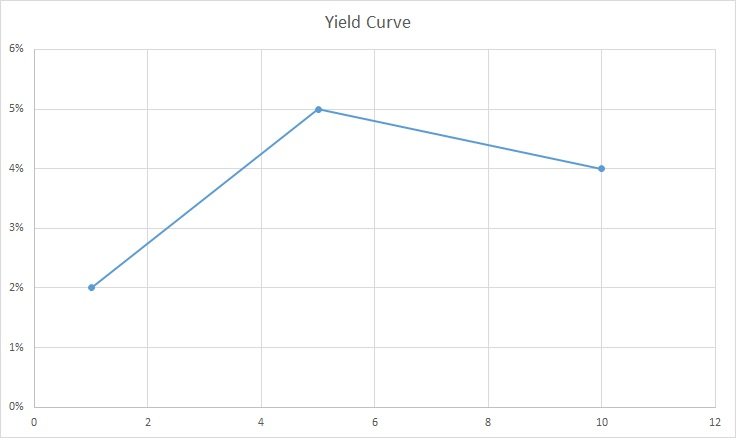
\includegraphics[width=3in]{figures/hump_shaped_yield_curve.jpg}
\end{center}
You are surprised by the hump shape, as yield curves are usually monotonically increasing.  Construct a zero-cost trading strategy that bets on the yield curve becoming monotonically increasing, but does not bet on the overall level of the yield curve.
}

\note{

}

\frame{\frametitle{Betting on Yield Curve Shapes}
\underline{Identify your view}:\\
Which bond(s) do you buy?  Which bond(s) do you short?  Explain.

\vspace{2.5in}

}

\note{
\begin{itemize}
\item Essentially, you view the 5-year bond yield as too high relative to the 1-year bond and 10-year bond.
\item Remember that yields and prices are inversely related.  So, you view the 5-year bond as too cheap (relative to the other bonds).
\end{itemize}

}

\frame{\frametitle{Betting on Yield Curve Shapes}
Calculate the modified duration of the three bonds and write down your balance sheet.  Assume that your position in the 5-year bond (either long or short) is \$1 in market value.

\vspace{2.5in}

}

\note{
\begin{tabular}{l|ll}
Assets & \multicolumn{2}{c}{Liabilities}\\
5yr & 1yr & 10yr\\\hline
\$1 & \$x & \$z \\
$MD = \frac{5}{1.05} = 4.7619$ & $MD = \frac{1}{1.02} = 0.9804$ & $MD = \frac{10}{1.04} = 9.6154$
\end{tabular}

}

\frame{\frametitle{Betting on Yield Curve Shapes}
Set-up two constraints: (1) Modified Duration Constraint and (2) Zero Initial Cash Outlay Constraint.  Solve for the market values of the 1-year and 10-year bond positions.

\vspace{2.25in}

Answer: \$0.5621 in 1yr, \$0.4379 in 10yr
}

\note{
Modified Duration Constraint:
\begin{align*}
1(4.7619) = 0.9804 x + 9.6154 z
\end{align*}
Zero Initial Cash Outlay Constraint:
\begin{align*}
1 = x + z
\end{align*}
Solving for x and z:
\begin{align*}
x = 0.5621\\
z = 0.4379
\end{align*}

}

\frame{\frametitle{Betting on Yield Curve Shapes}
Keep in mind that all of the values solved for are market values.  Convert them to face values.  Write down a balance sheet of your positions.

\vspace{2.5in}
}

\note{
\begin{align*}
& 5yr: 1 = \frac{FV_{5yr}}{1.05^5} \Rightarrow FV_{5yr} = 1.2763\\
& 1yr: 0.5621 = \frac{FV_{1yr}}{1.02} \Rightarrow FV_{1yr} = 0.5733\\
& 10yr: 0.4379 = \frac{FV_{10yr}}{1.04^{10}} \Rightarrow FV_{10yr} = 0.6482
\end{align*}

\begin{center}
\begin{tabular}{l|ll}
Assets & Liabilities\\
5yr & 1yr & 10yr \\\hline
\$1 market value & \$0.5621 market value & \$0.4370 market value\\
\$1.2763 face value & \$0.5733 face value & \$0.6482 face value
\end{tabular}
\end{center}

}

\frame{\frametitle{Betting on Yield Curve Shapes}
Suppose that the level of the yield curve increases (we had no view on this), but the 5yr yield drops relative to the other yields.
\begin{center}
\begin{tabular}{lll}
T & yield & $\Delta$ yield\\\hline
1 & 5\% & +3\\
5 & 6\% & +1\\
10 & 7\% & +3\\\hline
\end{tabular}
\end{center}
Calculate the new value of your portfolio.

\vspace{1.25in}

Answer: 0.0782
}

\note{
The value of the portfolio is now,
\begin{align*}
\frac{1.2763}{1.06^5} - \frac{0.5733}{1.05} - \frac{0.6482}{1.07^{10}} = 0.0782
\end{align*}

}

\frame{\frametitle{Betting on Yield Curve Shapes}
Suppose instead that the level of the yield curve increases (we had no view on this), but the 5yr is unchanged relative to the other yields.
\begin{center}
\begin{tabular}{lll}
T & yield & $\Delta$ yield\\\hline
1 & 5\% & +3\\
5 & 8\% & +3\\
10 & 7\% & +3\\\hline
\end{tabular}
\end{center}
Calculate the new value of your portfolio.

\vspace{1.25in}

Answer: -0.01
}

\note{
\begin{align*}
\frac{1.2763}{1.08^5} - \frac{0.5733}{1.05} - \frac{0.6482}{1.07^{10}} = -0.013
\end{align*}
Note that there is a slight change in portfolio value since modified duration hedging is not perfect.

}

\frame{\frametitle{Betting on Yield Curve Shapes}
Suppose instead that the level of the yield curve increases (we had no view on this), but the 5yr yield increases relative to the other yields.
\begin{center}
\begin{tabular}{lll}
T & yield & $\Delta$ yield\\\hline
1 & 3\% & +1\\
5 & 8\% & +3\\
10 & 5\% & +1\\\hline
\end{tabular}
\end{center}
Calculate the new value of your portfolio.

\vspace{1.25in}

Answer: -0.0859
}

\note{
\begin{align*}
\frac{1.2763}{1.08^5} - \frac{0.5733}{1.03} - \frac{0.6482}{1.05^{10}} = -0.0859
\end{align*}
Yields moved in the opposite way of what we were betting on.

}

\end{document}